% -----------------------------------------------
% Template for ISMIR Papers
% 2021 version, based on previous ISMIR templates

% Requirements :
% * 6+n page length maximum
% * 10MB maximum file size
% * Copyright note must appear in the bottom left corner of first page
% * Clearer statement about citing own work in anonymized submission
% (see conference website for additional details)
% -----------------------------------------------

\documentclass{article}
\usepackage[T1]{fontenc} % add special characters (e.g., umlaute)
\usepackage[utf8]{inputenc} % set utf-8 as default input encoding
\usepackage{ismir,amsmath,cite,url}
\usepackage{float}
\usepackage{amssymb}
\usepackage[ruled]{algorithm2e}
\usepackage{cleveref}
\crefrangeformat{equation}{Eq.~(#3#1#4) to~(#5#2#6)}
\Crefrangeformat{equation}{Equations~(#3#1#4) to~(#5#2#6)}
\usepackage{graphicx}
\usepackage{subcaption}
\usepackage{color}
\usepackage{multirow}
\usepackage{enumitem}
\usepackage{tablefootnote}


\usepackage{lineno}
\linenumbers

% Title. Please use IEEE-compliant title case when specifying the title here,
% as it has implications for the copyright notice
% -----
\title{The power of deep without going deep? A study of HDPGMM music representation learning}

% Note: Please do NOT use \thanks or a \footnote in any of the author markup

% Single address
% To use with only one author or several with the same address
% ---------------
%\oneauthor
% {Names should be omitted for double-blind reviewing}
% {Affiliations should be omitted for double-blind reviewing}

% Two addresses
% --------------
%\twoauthors
%  {First author} {School \\ Department}
%  {Second author} {Company \\ Address}

% Three addresses
% --------------\input{ISMIR2021_paper.tex}

\threeauthors
  {First Author} {Affiliation1 \\ {\tt author1@ismir.edu}}
  {Second Author} {\bf Retain these fake authors in\\\bf submission to preserve the formatting}
  {Third Author} {Affiliation3 \\ {\tt author3@ismir.edu}}

% Four or more addresses
% OR alternative format for large number of co-authors
% ------------
%\multauthor
%{First author$^1$ \hspace{1cm} Second author$^1$ \hspace{1cm} Third author$^2$} { \bfseries{Fourth author$^3$ \hspace{1cm} Fifth author$^2$ \hspace{1cm} Sixth author$^1$}\\
%  $^1$ Department of Computer Science, University , Country\\
%$^2$ International Laboratories, City, Country\\
%$^3$  Company, Address\\
%{\tt\small CorrespondenceAuthor@ismir.edu, PossibleOtherAuthor@ismir.edu}
%}

% For the author list in the Creative Common license, please enter author names. 
% Please abbreviate the first names of authors and add 'and' between the second to last and last authors.
\def\authorname{F. Author, S. Author, and T. Author}

% Optional: To use hyperref, uncomment the following.
%\usepackage[bookmarks=false,pdfauthor={\authorname},pdfsubject={\papersubject},hidelinks]{hyperref}
% Mind the bookmarks=false option; bookmarks are incompatible with ismir.sty.

\sloppy % please retain sloppy command for improved formatting

\begin{document}

%
\maketitle
%
\begin{abstract}
    In the previous decade, Deep Learning (DL) has proven to be one of the most effective machine learning methods to tackle a wide range of Music Information Retrieval (MIR) tasks. It offers the highly expressive learning capacity that can fit any music representations in need for the downstream tasks, which sacrifices interpretability.
    On the other hand, the Bayesian nonparametric approach promises similar properties, such as the high flexibility while being robust to the overfitting and preserving the interpretability. The primary motivation of this work is to explore the potential of Bayesian nonparametric models in MIR tasks by focusing on the representation learning aspect especially compared to the DL models.
    We assess the music representation learned from the Hierarchical Dirichlet Process Gaussian Mixture Model (HDPGMM), an infinite mixture model based on the Bayesian nonparametric approach, to MIR tasks, including classifications, auto-tagging, and recommendation.
    The experimental result suggests that the HDPGMM music representation can outperform DL representations in certain scenarios, and overall comparable.
\end{abstract}
%
\section{Introduction}\label{sec:introduction}

% Skeleton
% - DL is the major tool to do various MIR tasks (classification / generation / recommendataion / etc.)
%   - It seems obvious as DL provides:
%     1. flexibility / expressiveness -> fit anything
%     2. means to fight against overfitting (regularizations) -> generalizes fine
%     3. infrastructure (hardware acceleration / software ecosystem) -> fast and easy to do
%   - one of the major benefits of DL (based on these properties) is that it can learn useful latent representation from the data automatically.
% - It's not perfect though, and one of the criticisms that would apply to DL is the lack of transparency.
% - There are some other paradigms beyond DL, that tries to achieve similar goals.
% - Bayesian Nonparametric models can be seen as one of those methodologies.
%   - Its premises are:
%     1. as a non-parametric model, it achieves the necessary expressiveness
%     2. as a Bayesian model, it inherently is robust against the overfitting
% - One good example would be the infinite mixture model, where the model find the right size of the component that fits to the dataset, which often needs some manual search procedure such as the cross validation.

Deep Learning (DL) became one of the most popular and successful methodologies to tackle a various range of Music Information Retrieval (MIR) tasks; music classification~\cite{musicclassification:book}, music generation~\cite{briot2019deep}, recommendation~\cite{10.3389/fams.2019.00044} and more. Some of the known benefits are: 1) the high flexibility towards any data structure and expressiveness, 2) effective ways to handling the overfitting at the same time, and finally 3) the rapidly improving infrastructural supports, including both hardwares (i.e., accelerators such as GPU) and softwares (i.e., deep learning frameworks).

Fuelled by these benefits, DL models can learn useful representation of the diverse data structures, which is one of the key reasons of its success~\cite{DBLP:conf/ismir/HumphreyBL12}. At its cost, on the other hand, DL models often are criticized by its opacity and the lack of interpretability~\cite{DBLP:conf/dsaa/GilpinBYBSK18}, which also holds for the applications within MIR domain~\cite{DBLP:journals/tmm/Sturm14,DBLP:journals/cie/Sturm16}.

The Bayesian nonparametric approach is an alternative approach to achieve what DL does well in an interpretable way. As a non-parametric method, it can overcome the underfitting by unlimited model capacity, while resisting against the overfitting with its Bayesian nature~\cite{DBLP:reference/ml/Teh17}. At the same time, the model can be interpretable through its probabilistic model structure itself, as the modelling procedure is to state, or infer the data generation process in the first place.

Bayesian nonparametric models have been applied in various MIR tasks for previous decades. As latent representation of music audio, it was applied to esitimate music (self) similarity~\cite{DBLP:conf/icassp/QiPC07, DBLP:conf/ismir/HoffmanBC08}. It also was employed to conduct harmonic and spectral analyses by decomposing the time-frequency representation of the music audio into the mixture of infinite latent components~\cite{Hoffman09findinglatent, DBLP:conf/icassp/NakanoRKOS11}. These analyses also have shown to be useful for downstream tasks such as the structural analysis~\cite{DBLP:conf/icassp/NakanoOKMK12} or music recommentation~\cite{DBLP:conf/ismir/YoshiiG09}. Further, discriminative model based on the Bayesian nonparametric is developed for the music emotion recognition~\cite{DBLP:journals/taffco/WangLCCH15}.

In spite of the similar premises they propose, however, Bayesian nonparametric models have not yet gained as much attention as DL recieved in MIR field. To our best knowledge, in particular, they have not been compared under similar experimental control within MIR context. As they promise quite similar high-level properties, it would be worth to explore to what extent they compare.

The research goal of this work is to assess the music representation learned from Bayesian nonparametric models by comparing them to the modern deep neural network models. In particular, we consider the Hierarchical Dirichlet Process Gaussian Mixture Model (HDPGMM)~\cite{DBLP:journals/jmlr/WangPB11,DBLP:conf/ismir/YoshiiG09,doi:10.1198/016214506000000302} as our model of interest. The comparison can confirm the potential of Bayesian nonparametric models as a representation learner over the DL methods.
To concretize the comparison, we employ the transfer learning experimental framework
~\cite{DBLP:journals/nca/KimULH20, DBLP:conf/ismir/ChoiFSC17, DBLP:conf/ismir/DielemanBS11}, which is commonly used for assessing the potential of representation itself. The contribution of this work can be listed as follows:

\begin{enumerate}
    \item We explore and suggest insight how ``good'' the music representation learned by Bayesian nonparametric models is under a range MIR tasks.
    \item We provide an efficient, GPU accelerated inference algorithm for HDPGMM, which can handle relatively scaled data.
\end{enumerate}

The remaining of the paper will present the HDPGMM (Section~\ref{sec:hdpgmm}), and discuss the experimental setup (Section~\ref{sec:experimental_setup}), followed by its result and discussion (Section~\ref{sec:result_discussion}). Lastly, we conclude the paper with a few pointers for the future works (Section~\ref{sec:conclusion}).


\section{HDPGMM}\label{sec:hdpgmm}

In this subsection, we introduce the main model we employ for this study, the Hiararchical Dirichlet Process Gaussian Mixture Model (HDPGMM)~\cite{DBLP:conf/ismir/HoffmanBC08, doi:10.1198/016214506000000302}. We first discuss the Dirichlet Process Mixture Model (DPMM), the model on which HDPGMM is extended.

\subsection{Dirichlet Process Mixture Models}\label{sec:hdpgmm:dpmm}

Mixture models such as GMMs assume a finite number of components from which each of observed feature vectors are drawn. It is well known that finding the optimal number $K$ of the mixuture components is a difficult problem. There are a few approaches that can be useful to estimate $K$ such as using the cross-validation. Dirichlet Process Mixture Model (DPMM) circumbents this problem by parametrizing the number of mixtures as part of the model. DP plays a central role for such models.

DP is a stochastic process which draws random probability distributions. Due to this property, it is often described as a distribution over distributions~\cite{DBLP:reference/ml/Teh17}. It can be also seen as the infinite dimensional generalization of the Dirichlet distributions~\cite{DBLP:reference/ml/Teh17}.
This aspect is the core building block of the Bayesian non-parametric models such as infinite mixture models. Setting DP as a prior distribution for the responsibility $\pi$ (also often referred as mixture probability) of mixture components allows the mixture model to infer both the relative weight among components and the appropriate number of maximum components for given observations.

Among a several ways to represent DP, we introduce the stick-breaking construction~\cite{sethuraman94}.
\footnote{Literature commonly chooses the Chinese Restaurant Process (CRP) for a illustrative metaphor for DP as it is intuitive and well explains various properties of DP~\cite{DBLP:reference/ml/Teh17}. We mainly discuss DP with the stick-breaking construction due to its further usage in the model inference within the work. For readers interested in other metaphorical descriptions of DP, we kindly refer them to~\cite{DBLP:reference/ml/Teh17, DBLP:conf/ismir/HoffmanBC08}}
Stick-breaking constructs DP in a simple and general manner. Formally, it is as follows:
\begin{equation}\label{eq:stick_breaking}
\begin{aligned}[c]
    \beta^{\prime}_{k} &\sim \text{Beta}(1, \gamma) \\
    \beta_{k} &= \beta^{\prime}_{k} \prod_{l=1}^{k-1} (1 - \beta_{l}^{\prime})
\end{aligned}
\qquad
\begin{aligned}[c]
    \phi_{k} &\sim H \\
    G_{0} &= \sum^{\infty}_{k=1} \beta_{k}\delta_{\phi_{k}}
\end{aligned}
\end{equation}
where two euqations in the left column represent the draw of infinite dimensional weight $\beta_{k}$ which sums to one. Notably, the distribution for $\beta$ is also referred as $\beta \sim \text{GEM}(\gamma)$~\cite{DBLP:journals/cpc/Pitman02}. In the right column, $H$ denotes the base distribution from which variable $\phi_{k}$ lying in some space $\Phi$ is drawn. The right bottom equation defines the draw of the probability measure $G_{0}$, where $\delta_{\phi_{k}}$ means the point mass centered at the component $\phi_{k}$. Altogether, Eq. \ref{eq:stick_breaking} constructs the DP $G_{0} \sim \text{DP}(\gamma, H)$. Figure \ref{fig:stick_breaking} depicts the process in graphical way.
\begin{figure}[ht]
    \centering
    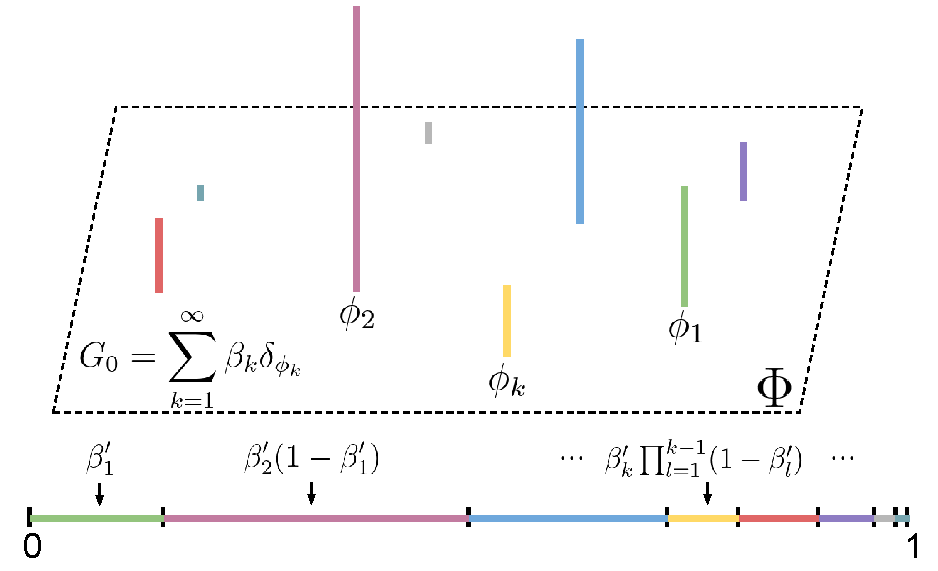
\includegraphics[width=0.9\linewidth]{figs/stick-breaking.pdf}
    \caption{Illustration of stick-breaking construction in Eq. \ref{eq:stick_breaking}}
    \label{fig:stick_breaking}
\end{figure}
In mixture model context, we want to infer mixture components $\{\phi_{1}, \phi_{2}, \cdots, \phi_{k}, \cdots\}$ that fits to the data observations $\{x_{1}, x_{2}, \cdots, x_{n}\}$, which are assumed to be drawn from distributions $F(\phi)$ parameterized with variable $\phi$ (i.e., mean and covariance $\phi = \{\mu, \Sigma\}$ in case of the multivariate Gaussian $F$). we can now use DP to draw $\phi$ as $i$th mixture components corresponds to the $i$th observation $x_{i}$ by introducing the cluster assignment variable $y_{i} \sim \text{Mult}(\beta)$:
\begin{equation}\label{eq:dpmm}
\begin{aligned}[c]
    \beta|\gamma &\sim \text{GEM}(\gamma) \\
    y_{i}|\beta &\sim \text{Mult}(\beta)
\end{aligned}
\qquad
\begin{aligned}[c]
    \phi_{k}|H &\sim H \\
    x_{i}|y_{i},\{\phi_{k}\} &\sim F(\phi_{y_{i}}) 
\end{aligned}
\end{equation}
where $\phi_{y_{i}}$ denotes the component parameter $\phi$ indexed by assignment variable $y_{i}$ corresponding to the $i$th observation $x_{i}$.

\subsection{Hierarchical DPMM}\label{sec:hdpgmm:hdpmm}

In many data structure, groupings of atomic data points arise naturally (i.e., audio frames within a song, songs from an artist, words of a lyrics). Hierarchical DP (HDP) is an extention of DP modelling ``groupings'' by imposing group-level DPs derived from the ``global-level'' or ``corpus-level'' DP as the global pool of components~\cite{doi:10.1198/016214506000000302}. Following Sethuraman's stick-breaking construction~\cite{DBLP:journals/jmlr/WangPB11}, $j$th group-level DP can be expressed as follows:
\begin{equation}\label{eq:hdp_doc_level}
\begin{aligned}[c]
    \pi^{\prime}_{jt} &\sim \text{Beta}(1, \alpha_{0}) \\
    \pi_{jt} &= \pi^{\prime}_{jt} \prod^{t - 1}_{l = 1} (1 - \pi^{\prime}_{jl})
\end{aligned}
\qquad
\begin{aligned}[c]
    \psi_{jt} &\sim G_{0} \\
    G_{j} &= \sum^{\infty}_{t = 1} \pi_{jt}\delta_{\psi_{jt}}
\end{aligned}
\end{equation}
As seen above, HDP indeed appears as the recursion of multiple levels of DPs\footnote{It implies naturally that multiple levels are possible (i.e., corpus - author - document), if it suits to the data structure.}. Notably, the base distribution $G_{0}$ of each group-level DP is from the corpus-level DP. This relationship allows to map group-level atoms $\psi_{jt}$ to the corpus-level atoms $\phi_{k}$. Wang et al. introduce a series of indicator variables $c_{jt}$ which maps $\psi_{jt}$ and $\phi_{k}$ as follows\cite{DBLP:journals/jmlr/WangPB11}:
\begin{equation}\label{eq:psi2phi}
\begin{aligned}
    c_{jt} &\sim \text{Mult}(\beta) \\
    \psi_{jt} &= \phi_{c_{jt}}
\end{aligned}
\end{equation}
where $\beta$ is drawn from the corpus-level DP in Eq. \ref{eq:stick_breaking}. It simplifies the model as we do not need to explicitly represent $\psi_{jt}$~\cite{DBLP:journals/jmlr/WangPB11}.
Finally, we can represent HDPMM by introducing another indicator variable $z_{jn} \sim \text{Mult}(\pi_{j})$ for $n$th observation $x_{jn}$ within the $j$th group, similarly to Eq. \ref{eq:dpmm}:
\begin{equation}\label{eq:hdpmm}
\begin{aligned}[c]
    \pi_{j}|\alpha_{0} &\sim \text{GEM}(\alpha_{0}) \\
    z_{jn}|\pi_{j} &\sim \text{Mult}(\pi_{j})
\end{aligned}
\qquad
\begin{aligned}[c]
    \theta_{jn} = \psi_{jz_{jn}} &= \phi_{c_{jz_{jn}}}  \\
    x_{jn}|z_{jn}, c_{jt}, \{\phi_{k}\} &\sim F(\theta_{jn}) 
\end{aligned}
\end{equation}
where we use the indicator $z_{jn}$ to select $\psi_{jt}$, which eventually is mapped as $\phi_{c_{jz_{jn}}}$ that represents the parameter $\theta_{jn}$ to draw the observation $x_{jn}$. HDPGMM is then defined by simply setting $F$ as the (multivariate) Gaussian distribution and $H$ as one of distribution from which we can sample the mean and covariance (i.e., Gaussian-inverse Wishart distribution). Figure \ref{fig:hdpmm} depicts the HDPGMM graphically.
\begin{figure}[ht]
    \centering
    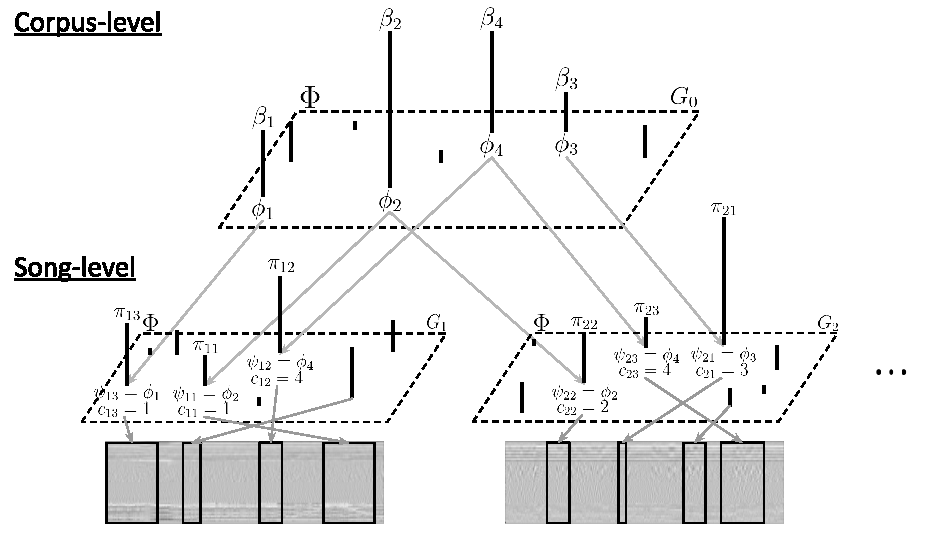
\includegraphics[width=\linewidth]{figs/HDP-stick-breaking.pdf}
    \caption{Illustration of 2-level HDPMM within corpus-song context. The top illustration depicts the corpus-level DP similar to Figure \ref{fig:stick_breaking}. The second row illustrations describe the draw of second level (song-level) DPs per song from the corpus-level DP. DPMM assumes that song features are drawn from each song-level DPs as depicted in the third rows of the image.}
    \label{fig:hdpmm}
\end{figure}


\subsection{Inference Algorithm}\label{sec:hdpgmm:inference}

In this section we discuss the inference (training) algorithm. We employ the online Variational Inference (VI)~\cite{DBLP:journals/jmlr/WangPB11}. VI is one of the common choices to infer a fully Bayesian models and usually significantly faster than other methods such as Markov Chain Monte Carlo (MCMC) with the expense of its relative precision. VI seeks the simpler, approximated version of the true posterior by minimizing the Kullback-Leibler (KL) divergence between approximation $q(Z)$ and the true posterior $p(Z|X)$, where $Z$ denote the set of latent variables and parameters that we want to find, and $X$ refers a set of observations~\cite{DBLP:journals/jei/BishopN07}.
% TODO: add bit more about the VI being approximating posterior (i.e., ln p(X) = L(q) + KL(q||p))
% p(Z|X) : posterior for variables Z
% p(X) : model evidence
% q(Z) : approximated posterior, which we'll set as fully-factorized one for the mean-field method
% TODO: do we need to be more explicit about these?
One of the popular simpliciation is full-factorization of the distribution $q(Z) = \prod^{|Z|}_{i=1} q_{i}(Z_{i})$. In the context of HDPGMM, we have the following factorization:
\begin{equation}\label{eq:meanfield_vi_hdpgmm}
    q(\beta^{\prime}, \pi^{\prime}, c, z, \phi) = q(\beta^{\prime})q(\pi^{\prime})q(c)q(z)q(\phi)
\end{equation}
where $\beta^{\prime}, \pi^{\prime}, c, z$ denote the corpus-level and group-level stick proportion, group-level component selection variable, and finally the observation-level component selection variable, respectively. $\phi$ refers the parameter(s) for the $F$ which draws the atomic observation, which is set as (multivariate) Gaussian in our context. Thus, $\phi$ includes the means $\mu$ and precision matrices $\Lambda$ of each Gaussian component\footnote{We adopt the result from \cite{DBLP:journals/jei/BishopN07}, where the Gaussian-Wishart distribution is used for the prior.}. 

Each variational distributions further factorize as follows:
\begin{equation}\label{eq:meanfield_further}
\begin{aligned}
    q(\beta^{\prime}) &= \textstyle \prod\nolimits_{k}^{K-1}\text{Beta}(\beta^{\prime}_{k}|u_{k}, v_{k}) \\
    q(\pi^{\prime}) &= \textstyle \prod\nolimits_{t}^{T-1}\text{Beta}(\pi^{\prime}_{t}|a_{t}, b_{t}) \\
    q(c) &= \textstyle \prod\nolimits_{j}\prod\nolimits_{t}\text{Mult}(c_{jt}|\varphi_{jt}) \\
    q(z) &= \textstyle \prod\nolimits_{j}\prod\nolimits_{n}\text{Mult}(z_{jn}|\zeta_{jn}) \\
\end{aligned}
\end{equation}
where $u_{k}, v_{k}, a_{t}, b_{t}$ denote the variational parameters for the Beta distributions for corpus-level and group-level stick proportions, respectively. $\varphi_{jt}\in\mathbb{R}^{K}, \zeta_{jn}\in\mathbb{R}^{T}$ are the variational parameters for the Multinomial distribution to draw the selector $c$ and $z$.

Notably, we truncate the inifinite Beta distributions by $K$ and $T$, which is a common method for applying VI on the infinite mixture model. With sufficiently large number for the truncation, the model will still not be limited to the truncation, and will only use the number of components that suits for given dataset. Final variational distribution is the Gaussian-Wishart prior distribution which draws the Gaussian parameters $\phi = \{\mu, \Lambda\}$ for distribution $F$:
\begin{equation}\label{eq:meanfield_normalwishart}
    q(\phi) = \textstyle \prod\nolimits_{k}^{K}\mathcal{N}(\mu_{k}|m_{k}, (\lambda_{k}\Lambda_{k})^{-1})\mathcal{W}(\Lambda_{k}|W_{k}, \nu_{k})
\end{equation}
where we draw the precision $\Lambda_{k}\in\mathbb{R}^{d \times d}$ from Wishart distribution with the variational parameter $W_{k}\in\mathbb{R}^{d \times d}$ and $\nu_{k}\in\mathbb{R}$, and the mean $\mu_{k}\in\mathbb{R}^{d}$ is drawn by the precision weighted by $\lambda_{k}\in\mathbb{R}$ and mean $m_{k}\in\mathbb{R}^{d}$.

We then can obtain the optimal model by maximizing the lowerbound of the marginal log likelihood $\text{log}\,p(X|Z)$~\cite{DBLP:journals/jei/BishopN07, DBLP:journals/ml/JordanGJS99, 10.1214/06-BA104}:
\begin{equation}\label{eq:lowerbound}
\begin{aligned}
    \text{log}\, p(X|Z) \geq \mathbb{E}_{q}[\text{log}\,p(X, \beta^{\prime}, \pi^{\prime}, c, z, \phi)] + H(q) \\
    = \textstyle \sum_{j} \big\{ \mathbb{E}_{q}[\text{log}\,(p(X_{j}|c_{j}, z_{j}, \phi)p(c_{j}|\beta^{\prime})p(z_{j}|\pi_{j}^{\prime})p(\pi^{\prime}_{j}|\alpha_{0}))] \\
    + H(q(c_{j})) + H(q(z_{j})) + H(q(\pi^{\prime}_{j})) \big\} \\
    + \mathbb{E}_{q}[\text{log}\,p(\beta^{\prime})p(\phi)] + H(q(\beta^{\prime})) + H(q(\phi))
\end{aligned}
\end{equation}
where $H(\cdot)$ denotes the entropy of given distribution, and $X_{j} = \{x_{j1}, x_{j2}, \cdots, x_{jN_{j}}\}$ is a set of observations within $j$th group.\footnote{Thus, the terms inside the sum over the group would further factorized into sums of these per-group observation. We omit them to avoid the equation being too crammed.}

Using the standard result of VI~\cite{DBLP:journals/jei/BishopN07, 10.1214/06-BA104, DBLP:journals/jmlr/WangPB11}, the update rules for group-level parameters are dreived as follows:
\begin{align}
\label{eq:doc_update:a} a_{jt} &= \textstyle 1 +  \sum_{n}\zeta_{jnt} \\
\label{eq:doc_update:b} b_{jt} &= \textstyle \alpha_{0} +  \sum_{n}\sum^{T}_{s=t+1}\zeta_{jnt} \\
\label{eq:doc_update:varphi} \varphi_{jtk} &\propto \text{exp}(\textstyle \sum_{n}\zeta_{jnt}\mathbb{E}_{q}[\text{log}\,p(x_{jn}|\phi_{k})] + \mathbb{E}_{q}[\text{log}\,\beta_{k}]) \\
\label{eq:doc_update:zeta} \zeta_{jnt} &\propto \text{exp}(\textstyle \sum_{k=1}^{K} \varphi_{jtk} \mathbb{E}_{q}[\text{log}\,p(x_{jn}|\phi_{k})] + \mathbb{E}_{q}[\text{log}\,\pi_{jt}])
\end{align}
Similarly, the update rules for the corpus-level parameters are as follows~\cite{DBLP:journals/jei/BishopN07}:
\begin{align}
\label{eq:corpus_update:u} u_{k} &= 1 + \textstyle \sum_{j}\sum_{t=1}^{T} \varphi_{jtk} \\
\label{eq:corpus_update:v} v_{k} &= \gamma + \textstyle \sum_{j}\sum_{t}^{T}\sum_{l=k+1}^{K} \varphi_{jtl} \\
\label{eq:corpus_update:lambda} \lambda_{k} &= \lambda_{0} + N_{k} \\
\label{eq:corpus_update:m} m_{k} &= \lambda_{k}^{-1} (\lambda_{0}m_{0} + N_{k}\bar{x}_{k}) \\
\label{eq:corpus_update:W} W_{k}^{-1} &= W_{0}^{-1} + N_{k}S_{k} + \frac{\lambda_{0}N_{k}}{\lambda_{0} + N_{k}} (\bar{x}_{k} - m_{0})(\bar{x}_{k} - m_{0})^{\intercal} \\
\label{eq:corpus_update:nu} \nu_{k} &= \nu_{0} + N_{k}
\end{align}
where $\lambda_{0}\in\mathbb{R}, m_{0}\in\mathbb{R}^{d}, \nu_{0}\in\mathbb{R}, W_{0}\in\mathbb{R}^{d\times d}$ are the hyperparameters corresponding to the weight, location, degrees of freedom, and scale of Gaussian-Wishart distribution. The sufficient statistics and expectations used above update rules are defined as follows:
\begin{align}\label{eq:expectations_and_suffstats}
    &\mathbb{E}_{q}[\text{log}\,\beta_{k}] = \mathbb{E}_{q}[\text{log}\,\beta_{k}^{\prime}] + \textstyle\sum_{l=1}^{k-1}\,\mathbb{E}_{q}[\text{log}\,(1 - \beta_{l}^{\prime})] \nonumber\\
    &\mathbb{E}_{q}[\text{log}\,\beta_{k}^{\prime}] = \Psi(u_{k}) - \Psi(u_{k} + v_{k}) \nonumber\\
    &\mathbb{E}_{q}[\text{log}\,(1 - \beta_{k}^{\prime})] = \Psi(v_{k}) - \Psi(u_{k} + v_{k}) \nonumber\\
    &\mathbb{E}_{q}[\text{log}\,\pi_{jt}] = \mathbb{E}_{q}[\text{log}\,\pi_{jt}^{\prime}] + \textstyle\sum_{s=1}^{t-1}\,\mathbb{E}_{q}[\text{log}\,(1 - \pi_{s}^{\prime})] \nonumber\\
    &\mathbb{E}_{q}[\text{log}\,\pi_{jt}^{\prime}] = \Psi(a_{jt}) - \Psi(a_{jt} + b_{jt}) \nonumber\\
    &\mathbb{E}_{q}[\text{log}\,(1 - \pi_{jt}^{\prime})] = \Psi(b_{jt}) - \Psi(a_{jt} + b_{jt}) \nonumber\\
    &N_{k} = \textstyle\sum_{j}\sum_{n}\,r_{jnk} \nonumber\\
    &\bar{x}_{k} = \frac{1}{N_{k}}\textstyle\sum_{j}\sum_{n}\,r_{jnk}x_{jn} \nonumber\\
    &S_{k} = \frac{1}{N_{k}}\textstyle\sum_{j}\sum_{n}\,r_{jnk}(x_{jn} - \bar{x}_{k})(x_{jn} - \bar{x}_{k})^{\intercal} \nonumber
\end{align}
where $\Psi(\cdot)$ refers the digamma function, and $r_{jnk} = \sum_{t=1}^{T} \zeta_{jnt}\varphi_{jtk}$ is the inferred responsibility of $n$th observation of $j$th group on $k$th component. Standard batch update would compute statistics across the entire corpus, and updates the corpus level parameters. However, it may be slow or may suffer by too large or small numbers accumulated from a large scale corpus.

In this work, we employ the online VI where corpus-level parameters are updated per every group or mini-batch of group passed. In this way, the early phase of model inference can be accelerated substantially compared to the full-batch update~\cite{DBLP:journals/jmlr/WangPB11, DBLP:conf/nips/HoffmanBB10}. The corpus level update then contoled by the learning rate $\rho_{t} = (\tau_{0} + t)^{-\kappa}$, which is decayed over iterations controlled by the offset parameter $\tau_{0} > 0$ and scale $\kappa \in (0.5, 1]$:
\begin{equation}\label{eq:minibatch_update}
    Z_{t} = (1 - \rho_{t})Z_{t - 1} + \rho_{t}\tilde{Z}_{t}
\end{equation}
where $\tilde{Z}_{t}$ means one of the corpus-level parameter in \crefrange{eq:corpus_update:u}{eq:corpus_update:nu} updated by the given mini-batch at $t$th iteration, while $Z_{t-1}$ is the current parameter. To properly scale the update with respect to the mini-batch size, we weight them by the factor of $w = \frac{|\tilde{X}|}{|X|}$, where $|X|, |\tilde{X}|$ denote the number of groups within the entire observation set $X$ and the mini-batch of groups $\tilde{X}$.

Combining altogether, the overall inference algorithm is described in Algorithm \ref{alg:inference}.

\begin{algorithm}
\caption{Online VI for HDPGMM}\label{alg:inference}
Initialize $\mathbf{\phi}=(\phi_{k})^{K}_{k=1}$, $u=(u_{k})^{K}_{k=1}$, $v=(v_{k})^{K}_{k=1}$ randomly. Set $t=1$.\\
\While{Stopping critrion is not met}{
    Fetch a random mini-batch of groups $\tilde{X}$ \\
    \Repeat{mini-batch likelihood stops improving}{
        Update $a_{j}, b_{j}, \zeta_{j} \text{and} \varphi_{j}$ using \crefrange{eq:doc_update:a}{eq:doc_update:zeta}\\
    }
    Compute $u_{k}, v_{k}, \lambda_{k}, m_{k}, W_{k}, \text{and} \nu_{k}$ using \crefrange{eq:corpus_update:u}{eq:corpus_update:nu} \\
    Set $\rho_{t} = (\tau_{0} + t)^{-\kappa}$, $t \gets t + 1$ \\
    Update $u_{k}, v_{k}, \lambda_{k}, m_{k}, W_{k}, \text{and} \nu_{k}$ using Eq. \ref{eq:minibatch_update} 
}
\end{algorithm}

\subsection{Further Regularization}\label{sec:hdpgmm:regularization}

Inspired by the implementation of \cite{DBLP:journals/jmlr/WangPB11, 10.1214/06-BA104}, we apply the further regularization on the model. Specifically, we ``splash'' the uniform noise to the inferred responsibility $r_{jn}$ as it can be biased if the groups are corrupted or impcomplete, such as the preview audio of the entire song:
\begin{equation}\label{eq:additional_regularization}
    \tilde{r}_{jn} = (1 - \eta_{t}) r_{jn} + \eta_{t} e
\end{equation}
$\eta_{t}$ is the regularization coefficient that determines the extent uniform noise $e = (e_{k})_{k=1}^{K}$ is mixed into $r_{jn}$. $\eta_{t} = \frac{\eta_{0} * 10^{3}}{(t + 10^{3})}$ also is defined as decaying function similar to the learning rate $\rho_{t}$.


% \subsection{DPMMs in MIR}\label{sec:hdpgmm:in_mir}

%blahblah


\section{Experimental Setup}\label{sec:experimental_setup}

In this section, we discuss the details of the empirical experiment we conduct. The overall design is adopted from the recent music representation learning studies~\cite{DBLP:conf/ismir/ChoiFSC17,DBLP:journals/nca/KimULH20,DBLP:conf/ismir/SpijkervetB21}, where multiple downstream music machine learning tasks are tested with the feature set learned from the representation models.

\subsection{Datasets, Features \& Evaluation}\label{sec:experimental_setup:datasets_evaluation}

We used the subset of Million Song Dataset (\textbf{MSD})~\cite{Bertin-Mahieux2011} as the ``source'' dataset for the representation learning (i.e., inference for HDPGMM). Specifically, we used the preview music excerpts from the ``train'' subset of MSD introduced by~\cite{DBLP:conf/ismir/PonsNPSES18,app8010150}\footnote{Length of preview audio differs per clips, where about 70\% of samples are approximately 30 seconds and rest are 1 minute, with a small subset is longer than 1 minute.}.
For the evaluation of the representation, we employ three target (downstream) tasks encompassing \emph{music genre classification}, \emph{music auto tagging}, \emph{music recommendation}. For each target task, we chose the \textbf{GTZAN} dataset~\cite{DBLP:journals/taslp/TzanetakisC02} with the fault-filtered split~\cite{DBLP:journals/tmm/KereliukSL15}, MagnaTagaTune (\textbf{MTAT}) dataset~\cite{DBLP:conf/ismir/LawWMBD09} with the split from ~\cite{lee_multi-level_2017}, and finally the Echo Nest taste profile subset as part of MSD (\textbf{Echonest})~\cite{Bertin-Mahieux2011} filtered by user and item frequency~\cite{DBLP:conf/www/LiangKHJ18} for the genre classification, auto-tagging and recommendation, respectively.

The evaluation is done by the cross-validation of task-specific prediction models.
We fit the logistic regression models for GTZAN and MTAT dataset which takes learned music represetnation as input and predicts the genre or music tags respectively. We find the hyper-parameters of logistic regression model by the randomized parameter search~\cite{DBLP:journals/jmlr/BergstraB12} for each run.

As for the recommendation, we apply the item \emph{K} Nearest Neighbor (\emph{item-kNN}) method~\cite{DBLP:journals/tois/DeshpandeK04} where the song-song similarity is measured by the \emph{cosine simiarlity} of the learned music representation. We adopted the data split introduced in \cite{DBLP:conf/www/LiangKHJ18}.\footnote{For every trial, disjoint validation and test users are uniformly sampled, which includes $10\%$ of population for each. Then $30\%$ of listening records of these users are hold out as testing interactions. We find the best \emph{K} by conducting the grid search on the range $\textit{K}\in\{2^{4}, 2^{5}, 2^{6}, 2^{7}, 2^{8}, 2^{9}\}$ by measuring the accuracy on the validation users. Using the best \emph{K}, we compute final score on the testing user, holding out the same amount of the interaction. For each run, We take the average score over $5$ trials to incorperate the random split effect.}
We repeat $5$ ``runs'' for each of downstream evalution to take account the various random effect (i.e., initialization, randomized search). The accuracy performance of each target task is assessed by commonly used accuracy measure in each task, which are further elaborated in Table~\ref{tab:dataset}.

\begin{table}[h!]
\centering
\begin{tabular}{ cccc }
    \hline
    Id       & \# Samples & \# Classes   & Acc. Measure \\ 
    \hline
    \hline 
    MSD      & $213,354$ & N/A           & N/A          \\ 
    \hline
    GTZAN    & $1,000$   & $10$          & F1~\cite{DBLP:books/bu/Rijsbergen79} \\
    MTAT     & $25,863$  & $50$          & AUROC~\cite{DBLP:journals/prl/Fawcett06} \\
    Echonest & $40,980$  & $571,355$\tablefootnote{It refers the number of users in this dataset.} & nDCG~\cite{DBLP:journals/tois/JarvelinK02} \\
    \hline
\end{tabular}
\caption{Details on dataset used. We use \emph{macro} average strategy for F1 and Area Under Receiver Operating Characteristic curve (AUROC) measure, and we consider top $500$ recommendationed songs for computing the normalized Discounted Cumulative Gain (nDCG).}
\label{tab:dataset}
\end{table}

We select a set of audio features to infer the HDPGMM and non-DL baseline models inspired by~\cite{DBLP:journals/taffco/WangLCCH15}. The detailed curation of the features can be found in Table ~\ref{tab:feature}\footnote{We use the implementation of \texttt{librosa}~\cite{librosa_0_9_1} with the default parameters for all the features.}.

\begin{table}[h!]
\centering
\begin{tabular}{ cccc }
    \hline
    Feature       & Aspect   & Dim.   & Transform\\ 
    \hline
    \hline 
    MFCC & Timbre & 13 & -         \\ 
    $\Delta$MFCC & Timbre & 13 & -         \\ 
    $\Delta\Delta$MFCC & Timbre & 13 & -         \\ 
    Onset Strength\cite{88} & Rhythm & 1 & $\text{log}$  \\ 
    Chroma\cite{ellis_2007} & Tonal & 12 & $\text{log}$  \\ 
    \hline
\end{tabular}
\caption{Details on the base audio features we employed for the experiment.}
\label{tab:feature}
\end{table}

\subsection{Comparisons}\label{sec:experimental_setup:comparisons}

We evaluate $4$ comparisons against HDPGMM, which includes both DL based models and non-DL based models.

\begin{itemize}[noitemsep, leftmargin=*]
    \item \textbf{G1} is the simplist model among the comparison. The song-wise feature is represented by the concatenated parameters $\phi = \{\mu, \Sigma\}$ of the single multivariate Gaussian fitted on the frame-level base audio feature vectors within a song\footnote{We chose the diagonalized covariance, which means the feature is concatenation of \emph{mean} $\mu\in\mathcal{R}^{52}$ and \emph{standard deviation} $\sigma\in\mathcal{R}^{52}$ of features.}.

    \item \textbf{VQ Codebook} can be deemed as the simple approximation of HDPGMM models~\cite{DBLP:conf/ismir/HoffmanBC08}. First a corpus-wise $K$ means clustering model is fitted on the song features in the frame-level. Later song-level feature is represented by the normalized frequency of cluster assignment of each frame-level base audio feature vector within the song. It can be interpreted similarly to the inferred cluster assignment variable $\pi_{j}$ in Eq. (\ref{eq:hdpmm}). We set the number of cluster as $256$, same to the maximum number of corpus-level components $K$ of HDPGMM models.
        % As the number of corpus level cluster $K$ is a free parameter, we assess in total four variants $K \in \{32, 64, 128, 256\}$ to provide a comprehensive overview.

    \item \textbf{KIM} is a DL based music representation trained in a simple self-supervised learning framework~\cite{DBLP:journals/nca/KimULH20}. The objective function of the model is to measure the extent which a siamenese neural network~\cite{koch2015siamese} can predict whether the two song clips it takes are cropped from the same song or different songs. We use the original implementation of the work, which takes the stereo mel-spectrogram as input. The representation is extracted from the last hidden layer before the prediction, and summarized with global average and standard devication pooling, through the entire song excerpt.

    \item \textbf{CLMR}~\cite{DBLP:conf/ismir/SpijkervetB21} is recent DL based music representation employing the self-supervised learning through the contrastive learning method~\cite{DBLP:conf/icml/ChenK0H20}. We employed the original implementation of~\cite{DBLP:conf/ismir/SpijkervetB21} that uses the raw audio samples as input feature\footnote{Unlike the original work, we set the dimensionality of hidden layer where we extract the representation as $256$ to control the representation dimensionality with other comparisons. Also, we do not apply the data augmentation for a fair comparison and also as it is beyond the main scope of the work. However, as it is reported that it can meaningfully improve the representation, we assume that applying the method would benefit similarly to other models as well.}. The representation is drawn from the last hidden layer and pooled with global average over the entire song excerpt.

    \item \textbf{HDPGMM}\footnote{inference algorithm in \cref{alg:inference} is implemented on \texttt{PyTorch}~\cite{NEURIPS2019_9015}, and thus support GPU acceleration.} uses the base audio feature with the whitening following~\cite{DBLP:conf/ismir/NamHSS12}. As for song-level representation $y_{j}$, we employ the expectation $\tilde{y}_{jk} = \mathbb{E}_{q}[\text{log}\,p(X_{j}|c_{j}, z_{j}, \phi_{k})]$ and normalize them over components and the length of the clip $y_{jk} = N_{j}^{-1}\frac{\tilde{y}_{jk}}{\sum_{k^{\prime}=1}^{K}\tilde{y}_{jk^{\prime}}}$. We adopt most of the hyper-parameter setup found from previous work~\cite{DBLP:journals/jmlr/WangPB11}; we set the maximum number of components on the corpus level $K$ and the song level $T$ as $256$ and $32$ respectively, mini-batch size to $1024$, learning rate parameters $\kappa=0.6$ and $\tau_{0}=64$. We, however, explore the regularization rate $\eta_{0} \in \{10^{-4}, 10^{-3}, 10^{-2}, 10^{-1}\}$ and total corpus size $|X| \in \{2\times10^{3}, 2\times10^{4}, 213354\}$ to examine their effect on the representation.
\end{itemize}

For the learning based models (i.e., KIM, CLMR, HDPGMM), we repeated $3$ trials to incorporate any random effect of learning algorithms. Within a trial, we iterated the update for $100$ epochs. Further, we set the dimensionality of the representation is set to $256$, homogeneous accross all comparisons except $G1$. Finally, we take the logarithm of the representation $\hat{y_{j}} = \text{log}(\text{max}(y_{j}, 10^{-8}))$ if it is given as the probability simplex (i.e., VQCodebook, HDPGMM).


\section{Result and Discussion}\label{sec:result_discussion}

\subsection{Effect of learning factors}\label{sec:result_discussion:learning_factors}

Overall, we observe that the learning factors of HDPGMM can make a substantial difference. As Figure \ref{fig:effects} shows, the result suggests that the additional regularization in Eq (\ref{eq:additional_regularization}) generally effect positvely on the performance of all the downstream tasks we tested. It implies that the entire song inputs would likely improve the representation further, as the regularization crudely mask the effect of the missing data due to the preview clipping to some extent.

Further, we found that the number of training samples also have a rather clear positive effect on the performances. We measured the effect by repeately sub-sampling the MSD training data $5$ times in two different sizes mentioned in \ref{sec:experimental_setup:comparisons}, and conduct the same evalution routine as the full training set. The result shows that the positive effect is logarithmic, which suggest that to get a linear improvement in the performance, the representation should be learned with exponentially larger dataset.


\begin{figure}[h]
    \begin{subfigure}{\linewidth}    
        \centering
        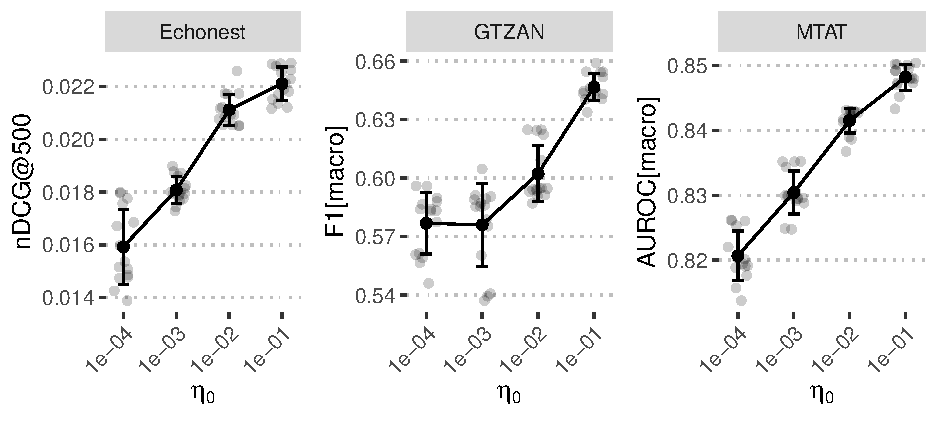
\includegraphics[width=\linewidth]{figs/regularization_effect.pdf}
        \caption{Effect of regularization factor $\eta_{0}$. ($|X| = 213,354$)}
        \label{fig:effects:regularization_effect}
    \end{subfigure}

    \begin{subfigure}{\linewidth}
        \centering
        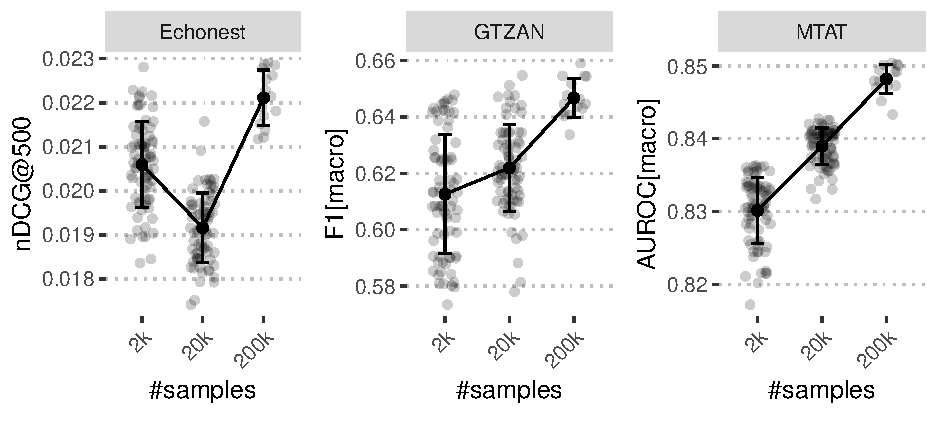
\includegraphics[width=\linewidth]{figs/num_sample_effect.pdf}
        \caption{Effect of the number of training samples. ($\eta_{0} = 10^{-1}$)}
        \label{fig:effects:num_samples_effect}
    \end{subfigure}
    \caption{Effect of the learning factors on HDPGMM. Error bar indicates the standard deviation, and grey dots are the raw datapoints.}
    \label{fig:effects}
\end{figure}

\subsection{Model Comparison}\label{sec:result_discussion:model_comparison}

\begin{table}[h]
\centering
\begin{tabular}{ c|l|c }
    \hline
    Dataset                 & Model         & Mean Acc.($\pm$SD)    \\ 
    \hline
    \hline 
    \multirow{5}*{Echonest} & G1            & 0.0252 ($\pm$ 0.0000) \\ 
                            & VQCodebook    & 0.0158 ($\pm$ 0.0000) \\
                            & KIM           & 0.0262 ($\pm$ 0.0012) \\
                            & CLMR          & \textbf{0.0279 ($\pm$ 0.0000)} \\
                            & HDPGMM        & 0.0224 ($\pm$ 0.0004) \\
    \hline
    \multirow{5}*{GTZAN}    & G1            & 0.5409 ($\pm$ 0.0000) \\ 
                            & VQCodebook    & 0.5776 ($\pm$ 0.0000) \\
                            & KIM           & 0.5448 ($\pm$ 0.0245) \\
                            & CLMR          & \textbf{0.6681 ($\pm$ 0.0000)} \\
                            & HDPGMM        & 0.6471 ($\pm$ 0.0059) \\
    \hline
    \multirow{8}*{MTAT}     & G1            & 0.8435 ($\pm$ 0.0000) \\ 
                            & VQCodebook    & 0.8373 ($\pm$ 0.0000) \\
                            & KIM           & 0.8021 ($\pm$ 0.0041) \\
                            & CLMR          & 0.8248 ($\pm$ 0.0000) \\
                            & HDPGMM        & \textbf{0.8452 ($\pm$ 0.0016)} \\
    \hline
\end{tabular}
\caption{Evaluation result on downstream tasks.}
\label{tab:main_result}
\end{table}

Model comparison result suggests that the HDPGMM model is comparable to the DL representation on average, and can be outperforming in a certain scenario. Reported in Table \ref{tab:main_result}, KIM achieves worse performance on GTZAN and MTAT than HDPGMM, while better at recommendation (Echonest). On the other hand, CLMR, which adopts a more sophisticated learning strategies, performed better in two tasks (GTZAN, Echonest) but still worse in the auto-tagging. It seems, however, Hierarchical mixture model variants (VQCodebook, HDPGMM) performs particularly worse in the recommendation task. We hypothesize that the cosine similarity might not be an optimal choice for the probability simplex representation, which however requires the further study.

Except this corner case, the HDPGMM representation outperforms the other non-DL comparisons in general. Especially, it achieves significant improvement over the simple version of it (VQCodebook) for all tasks, and mostly outperforming G1.


\subsection{Component Interpretability}\label{sec:result_discussion:interpretability}

\begin{table*}[h]
\centering
\small
\begin{tabular}{ ccccccc }
    \hline
    Hip-Hop & country & female vocalists & pop & electronic & pop & oldies \\
    pop & rock & singer-songwriter & female vocalists & dance & soul & blues \\
    rnb & pop & pop & female vocalist & electronica & female vocalists & country \\
    soul & oldies & acoustic & rock & funk & rnb & 60s \\
    male vocalists & indie & Mellow & Love & electro & dance & soul \\
    rock & singer-songwriter & folk & dance & Hip-Hop & Hip-Hop & rock \\
    hip hop & classic rock & female vocalist & female & House & rock & classic rock \\
    \hline
    $0.0394$ & $0.0308$ & $0.0299$ & $0.0269$ & $0.0268$ & $0.0248$ & $0.0227$ \\
    \hline
\end{tabular}
\caption{Top tags for a few mostly ``loaded'' components (column-wise). The last row is the normalized total responsibility $\tilde{N}_{k} = \frac{N_{k}}{\sum_{k^{\prime}}^{K} N_{k^{\prime}}}$, meaning the proportional amount of songs having the component.}
\label{tab:topic_tags}
\end{table*}

Finally, we 




\section{Conclusion and Future Works}\label{sec:conclusion}

%blahblah


% For bibtex users:
\bibliography{ISMIRtemplate}

\end{document}

